\section{Elgamal签名方案的实现}

\subsection{程序的模块划分}

我将程序划分为下面的三个基本模块:

\begin{figure}[H]
  \centering
  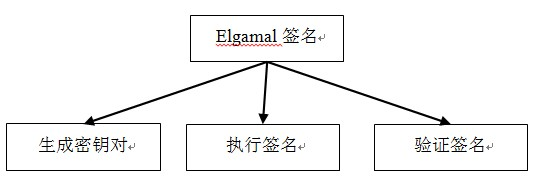
\includegraphics{img/1.jpg}
  \caption{ElGamal签名程序模块}
\end{figure}

\subsection{功能模块的具体实现}

\subsubsection{生成密钥对}

\begin{figure}[H]
  \centering
  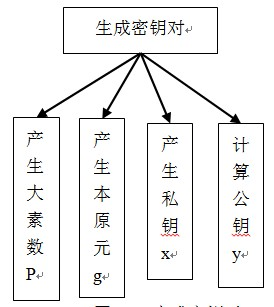
\includegraphics{img/2.jpg}
  \caption{生成密钥对}
\end{figure}

1)利用自定义函数void strongp(big p,int n,long seed1,long seed2)产生大素数$p$和$mod$ $p$ 下的本原元$g$

2)调用MIRACL库函数bigbits(64,x)随机生成64位的私钥$x$。并将$(x,g,p)$存入pri.txt,供签名时读取;

3)调用MIRACL库函数powmod(g,x,p,y)计算$y=g\textasciicircum x$ $mod$ $p$,得到公钥$y$,并将$(y,g,p)$存入pub.txt,供验证签名时读取。

\subsubsection{实现签名}

\begin{figure}[H]
  \centering
  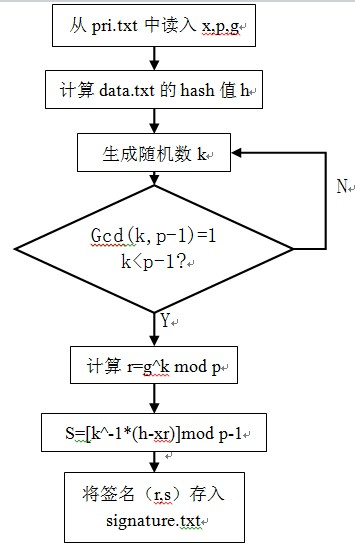
\includegraphics{img/3.jpg}
  \caption{签名流程图}
\end{figure}

1)  读取pri.txt文件中的$x$、$p$和$g$。

2)  计算h=messagehash1tobig();

3)  取随机数k要求k与p-1互素:
  decr(p, 1, p);                        // 临时:$p - 1$
  irand((unsigned int)time(NULL));
  while (egcd(p, k ,b\_tmp)!=1)
  {
    bigrand(p, k);
  }

4)  计算$r$:调用MIRACL库函数powmod(g,k,p,r)计算$r=g\textasciicircum k$ $mod$ $p$;

5)  计算$s$:使用函数decr(p, 1, p);使接下来的p都变为$p-1$进行运算;计算$k$逆元:xgcd(k,p,k,k,k);计算$x=x*r$, $h=h-x:multiply(r,x,x)$, subtract(h,x,h); 计算$s=[k\textasciicircum -1*(h-xr)]$ $mod$ $p-1$:$mad(k, h, h, p, p, s)$; 

6)  丢弃k:mirkill(k);

7)  将算得的签名$(r,s)$存入signature.txt中。

\subsubsection{验证签名}

1)    读取signature.txt中的签名$r$和$s$;

2)    计算data.txt的h,h=messagehash1tobig();

3)    计算$g\textasciicircum h(mod$ $p)$并将值存入$b_tmp_1$:powmod(g,h,p,$b_tem_1$);

4)    计算$y\textasciicircum r*r\textasciicircum s$ $(mod$ $p)$并将值存入$b_tmp_2$:powmod(y,r,r,s,p,$b_tmp_2$);

5)    比较$b_tmp_1$和$b_tmp_2$的值,若相等则签名正确,接受签名,反之签名错误,拒绝\cite{Provabl}\cite{jiyulisanduishu}。
